\section{Response Time}
\begin{itemize}
	\item TLS attacks still works and even better against DTLS for no RTT noise. 
\end{itemize}

\subsection{Different Sensors}
%Plaintext recovery.
%\begin{itemize}
%	\item Reading different sensors takes different time.
%	\item Requirement: needs to identify CoAPS packets.
%	\item Works on both 802.15.4 Seuciryt and DTLS, if the requirement is met. 
%\end{itemize}

CoAP\cite{rfc7252} is a protocol designed for constraied devices that provides an universal interface for accessing resources. CoAPs is the secure version which stands for CoAP with DTLS.

Due to the different physical characters of sensors, there could be a variance of time when reading the measurements. The idea is to investigate whether such variance can be observed through the packet response latency.

We implemented the experiment on CC2538, using all three sensors from ``cc2538-demo", namely Vdd, temperature and Ambient Light Sensor (ALS). We used CoAP from the ``er-rest-example" in the Contiki OS source code, as there is no CoAPs implementation available. 

Although DTLS processing would definitely have an impact on the response latency, we argue that such impact would be independent to the sensors being accessed; hence similar result would hold even in case of CoAPs.

We have carefully crafted other factors, including URIs, data representation and code flow, to be uniform for all three sensors in order to guarantee a controlled environment.

\begin{table}
	\center
	\begin{tabular}{|c|c|c|}
	\hline
	& Average (ms) & Range(ms) \\ 
	\hline
	Vdd & 9.622 & [9.388, 10.318] \\ 
	\hline
	Temperature & 9.835 & [9.525, 10.318] \\ 
	\hline
	ALS & 11.651 & [11.338, 12.031] \\
	\hline
\end{tabular} 
	\caption{CoAP Response Latency for Sensor Readings on CC2538\label{CoapTiming}}
\end{table}

\Cref{CoapTiming} summarises the result. It is shown that ALS takes about $2$ms longer and hence can be easily distinguished. Vdd and temperature might be difficult to distinguish by response latency as they have similar results.



\subsection{Different Hardware}
Gain hardware information.
\begin{itemize}
	\item Different hardware has different response latency against the same message.
	\item For 802.15.4: Requires additional information. Can be satisfied by the previous ICMP attack.
	\item For DTLS: No requirement. The adversary can actively send a message, e.g. PING.
\end{itemize}

A more general leakage is the response latency to a specific message, as different processors would have different computational power and thus different time to process a same message. The ICMP messages turns out to be suitable for this attack since they are standardised and thus universally supported. Among the ICMP messages, PING is especially ideal for two reasons: 
\begin{enumerate}
	\item It is mandatory in the ICMP standard.
	\item It only swaps the source and destination address of the packet; thus minimises different code path in protocol processing.
\end{enumerate}

\begin{table}
	\center
	\begin{tabular}{|c|c|c|}
	\hline
			& CC2538	& TelosB \\ 
	\hline
	Average(ms)	& 9.56		& 17.03 \\ 
	\hline
	Range(ms)	& [9.16, 10.06]	& [16.49, 17.68]	\\
	\hline
\end{tabular}

	\caption{PING Response Latency\label{PingResponse}}
\end{table}

\Cref{PingResponse} shows the PING response latency on CC2538 and TelosB. The result confirms that these devices can be distinguished by PING response latency.

\subsection{Running Code Fingerprint}
%Fingerprints the code running on a device, which leads to plaintext recovery.
%\begin{itemize}
%	\item Theory explained in \Cref{FingerprintTheory}.
%	\item Requirement: needs to actively send messages. Any Request/Response protocol works, such as PING, DTLS Heartbeat, CoAP PING, etc. 
%	\item Not for 802.15.4: adversary can't join the network.
%	\item For DTLS: PING is available and confirmed. DTLS Heartbeat should work if supported.
%\end{itemize}
The response time of packets can also be exploited to fingerprint the code running on a specific device. 

\begin{figure}
	\center
	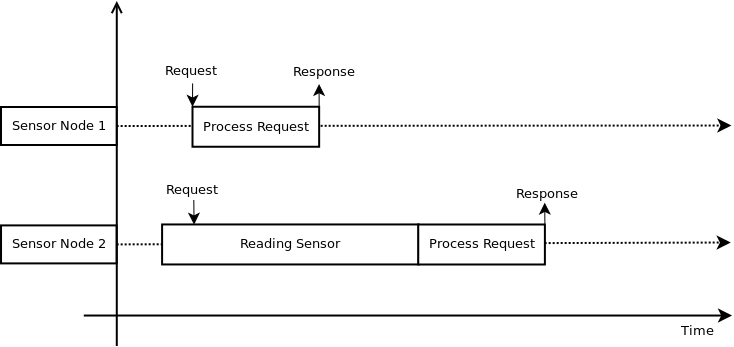
\includegraphics[width=\textwidth]{fig/PingProbe_Theory.png}
	\caption{Variations in PING Response Latency\label{FingerprintTheory}}
\end{figure}

%How it works
\Cref{FingerprintTheory} illustrates two sensors receiving a service request. The first node was idle and hence responded immediately, whilst the second postponed the request for reading a sensor. As a result, the response time on the second sensor would appear to be longer than the first sensor. This scenario applies to the majority of constrained devices as they are mostly single-cored. 

The idea of code fingerprinting exploits such extended response time. Since different task extends the response time differently, distributions of extended response time can be used as fingerprint to the code running on the device. The statistical distance between the distributions can therefore used as an indicator for matching the fingerprints.

%What can be the Request
To effectively launch the attack, the requests needs to be actively sent by the adversary. Since code information is actually contained in extended  length of response time; therefore requests with short constant processing time are preferable as they induce less noise. 

In practice, the request can be instantiated by several messages defined in the sensor network protocols. PING is ideal as it induces only negligible computation and is compulsory according to the ICMP standard\cite{rfc4433}. Other options include Heartbeat message in DTLS\cite{rfc6520}, Reset in CoAP\cite{rfc7252}, etc.

%Experiment Result